\section{Double-slit interference in \(T^2_{27}\): path memory, Born rule, and dodecaphasic unitarity}
\label{sec:md-sucesora-interferometria-t27}

The finite realization is constructed upon
\[
 \mathcal H_{\mathrm{cam}}
 =\ell^2\!\left(T_{27}^{2}\right)\otimes\mathbb C^4,
 \qquad
 T_{27}^{2}=(\mathbb Z/27\mathbb Z)^2,
\]
where the dimension factor \(4\) records the directions
\((N,S,E,W)\). Explicit memory of the trajectory adds the factor
\(\mathbb C^2_{\mathrm{mem}}\). The microscopic step is the operator
\begin{equation}
 U_{\mathrm{micro}}=S D_J C_4,
 \label{eq:md-sucesora-interferometro-microstep}
\end{equation}
with \(C_4\) unitary, \(D_J\) diagonal, and \(S\) as a shift conditioned
by direction. Consequently,
\[
 U_{\mathrm{micro}}^*U_{\mathrm{micro}}=I,
\]
and the norm is preserved at each step.

\subsection{Preparation of the \(2\) Trajectories and Reading Screen}

The two openings are fixed at
\[
 (x_0,y_1)=(2,8),
 \qquad
 (x_0,y_2)=(2,18),
\]
with the same initial directional state. If \(\psi_1\) and \(\psi_2\) are the
amplitudes propagated from each aperture, the screen located at \(x=24\)
publishes, for a real memory overlap \(\mu\in[0,1]\),
\begin{equation}
 I_\mu(y)
 =\frac12\sum_d
 \left(
  |\psi_1(24,y,d)|^2+|\psi_2(24,y,d)|^2
  +2\operatorname{Re}\!\left[
   \mu\,\overline{\psi_1(24,y,d)}\psi_2(24,y,d)
  \right]
 \right).
 \label{eq:md-sucesora-interferometro-intensidad}
\end{equation}
The formula is also obtained by introducing the markers
\[
 |m_1\rangle=(1,0),
 \qquad
 |m_2\rangle=(\mu,\sqrt{1-\mu^2})
\]
and tracing over \(\mathbb C^2_{\mathrm{mem}}\). This equality identifies the
overlap of the registers, rather than a loss of norm, as the origin of the
attenuation of the fringes. In particular,
\begin{equation}
 \mathcal V(\mu)=|\mu|\,\mathcal V(1).
 \label{eq:md-sucesora-interferometro-visibilidad}
\end{equation}
For \(\mu=0\), a phase correction cannot reconstruct the cross term;
if the markers are unmade unitarily before recombination, the
curve \(\mu=1\) is exactly recovered.

\subsection{Unitarity Identities of the Dodecaphase Order Under a Common Amplitude Budget}

The control block consists of \(12\) oriented pulses with zero vector
sum. The first \(6\) are obtained from a directional seed through
the dodecaphasic signature; the remaining \(6\) are their opposites.
Four sequences of \(36\) steps are compared:
\begin{enumerate}
 \item the canonical sequence, repeated for \(3\) full cycles;
 \item its oriented inverse;
 \item a sequence in which an opposite pair is replaced by common phases
       of the same norm;
 \item a random permutation of the same multiset of pulses.
\end{enumerate}
All preserve the pulse count, the null vector sum, and the quadratic
budget. The difference between their patterns therefore measures dependence
on noncommutative order and directional information, not an
unequal injection of norm or energy.

Noncommutativity is verified on a probe state fixed before the
reading:
\[
 \left\|U_bU_a\psi-U_aU_b\psi\right\|_2
 =0.24776388825652637.
\]
Numerical control provides
\[
 \|C_4^*C_4-I\|_{\max}=0,
 \qquad
 \max_t\bigl|\|\psi_t\|_2^2-1\bigr|
 =1.3322676295501878\times10^{-15},
\]
\[
 \Delta B_2=2.220446049250313\times10^{-16},
 \qquad
 \varepsilon_{\mathrm{Born}}
 =1.734723475976807\times10^{-18},
\]
\[
 \varepsilon_{\mathcal V(\mu)}
 =2.220446049250313\times10^{-16},
\]
where \(\Delta B_2\) is the maximum dispersion of the quadratic budget among
the four sequences.

\begin{table}[tbp]
\centering
\caption{Interference and distance from the canonical sequence after \(36\) steps.}
\label{tab:md-sucesora-interferometro-resultados}
\begin{tabular}{lccc}
\toprule
Sequence & \(\mathcal V_{\mathrm{lineal}}\) &
total variation distance & mean fidelity \\
\midrule
canonical      & \(0.5992212256\) & \(0\)            & \(1.0000000000\) \\
inverse       & \(0.5974219552\) & \(0.0333923142\) & \(0.9740951119\) \\
replaced pair& \(0.5907431085\) & \(0.0628288605\) & \(0.9417893564\) \\
randomized  & \(0.6254301808\) & \(0.0963185652\) & \(0.6564185376\) \\
\bottomrule
\end{tabular}
\end{table}

\subsection{Interference reconstructed at \(T^2_{27}\): detection distribution and physical domain}

\begin{theorem}[Unitary interference with explicit path memory]
For the dynamics defined by \eqref{eq:md-sucesora-interferometro-microstep},
the intensity obtained by tracing out the path record coincides with
\eqref{eq:md-sucesora-interferometro-intensidad}; the visibility satisfies
\eqref{eq:md-sucesora-interferometro-visibilidad}; and sequences with the same
quadratic budget may produce different patterns when their order
differs.
\end{theorem}

The proof is finite: unitarity of each factor, expansion of the square of the sum of the two branches, and partial contraction of the marker. The preceding numerical controls verify the run on \(T_{27}^{2}\). The concrete chart taking the dodecaphasic state to directional phases constitutes a declared physical realization; it is not identified by definition with the temporal return of \(108\) phases. The electron scale is applied after the dimensionless dynamics and neither selects the word nor fits the fringes.

The realization would be refuted by loss of unitarity, discrepancy between
the explicit memory and the Born rule, creation of interference by a phase
when \(\mu=0\), dependence of the energy budget on the sequence, or use
of the screen outcome to select the pulse order retrospectively.

\begin{figure}[tbp]
\centering
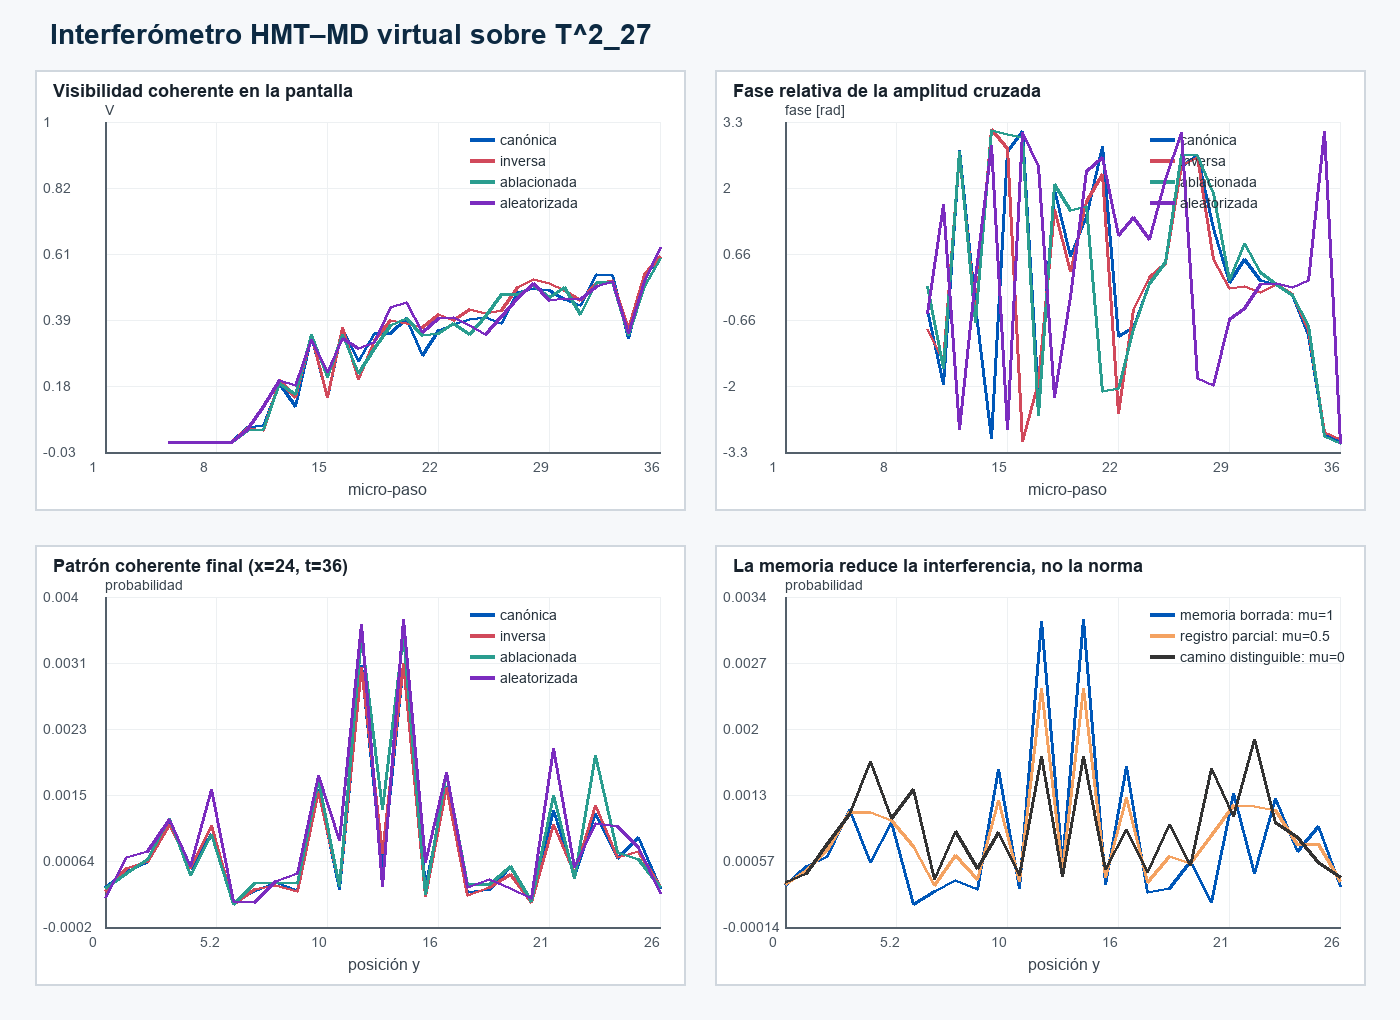
\includegraphics[width=.96\linewidth]{figures/parte_iv/01_curvas_y_patrones.png}
\caption[Evolution of visibility, relative phase, and final pattern]{Evolution of visibility, relative phase, and final pattern for the four sequences with common budget. The original image depicts the virtual HMT--MD interferometer on \(T^2_{27}\). Panel labels, from left to right and top to bottom: coherent visibility on the screen; relative phase of the cross amplitude; final coherent pattern \((x=24,t=36)\); memory reduces interference, not the norm. Axes: microstep, position \(y\), phase in radians, and probability. The four sequences are canonical, inverse, ablated, and randomized. The memory curves represent erased memory \((\mu=1)\), partial record \((\mu=0.5)\), and a distinguishable path \((\mu=0)\).}
\label{fig:md-sucesora-interferometro-patrones}
\end{figure}

\begin{figure}[tbp]
\centering
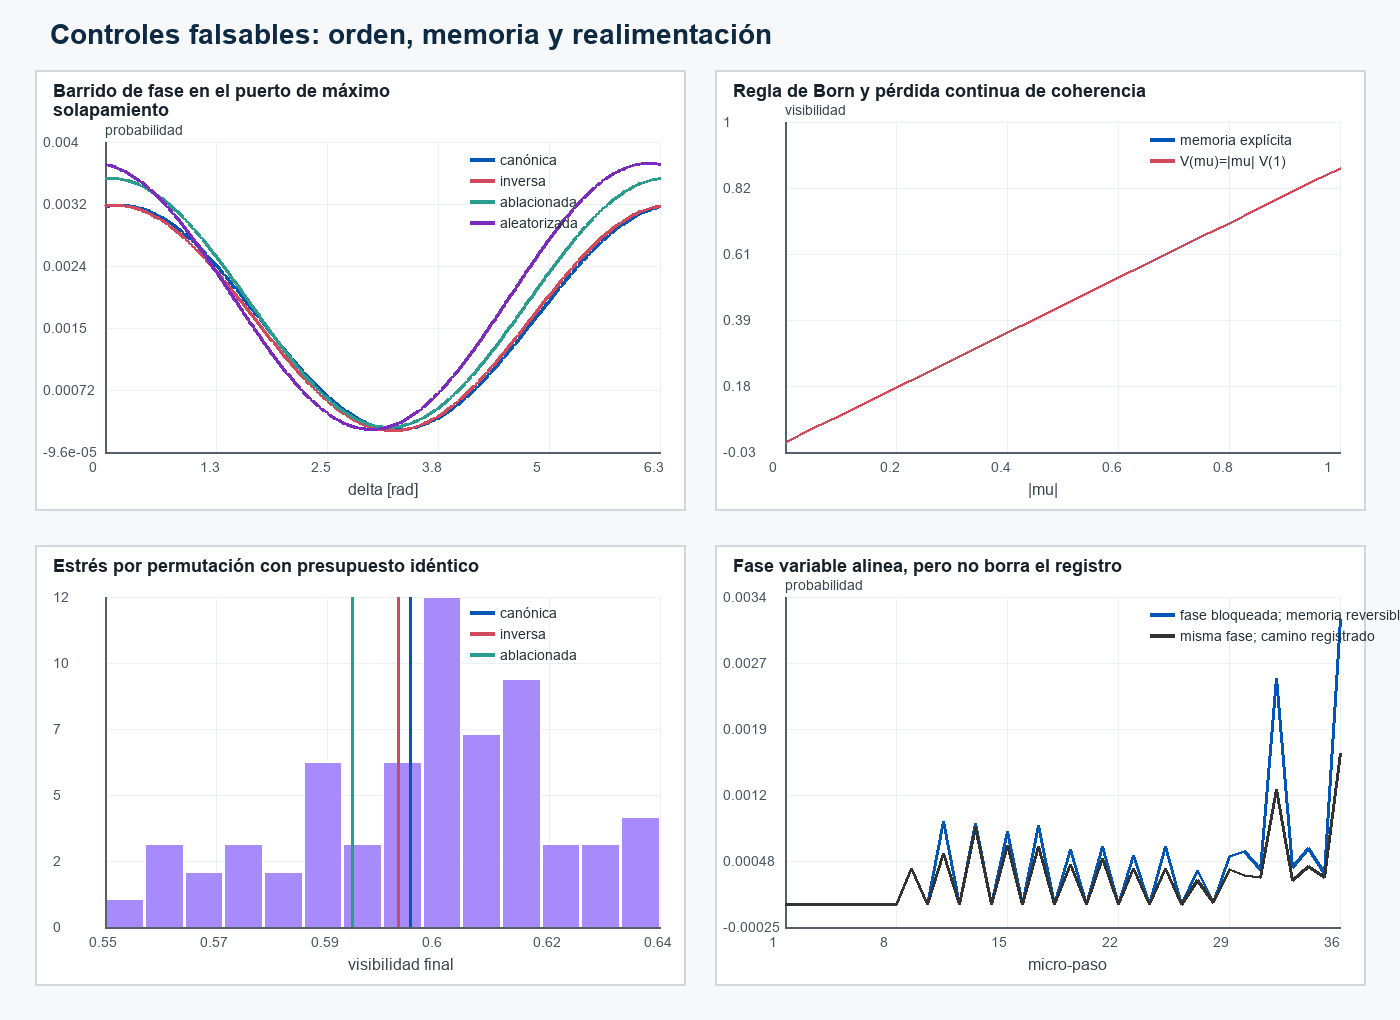
\includegraphics[width=.96\linewidth]{figures/parte_iv/02_estres_memoria_y_control.png}
\caption[Order controls, path memory, and phase feedback]{Order controls, path memory, and phase feedback. The original image presents falsifiable controls of order, memory, and feedback. Panel labels, from left to right and top to bottom: phase sweep at the port of maximum overlap; Born rule and continuous loss of coherence; permutation stress with an identical budget; variable phase aligns, but does not erase the record. Axes: probability, visibility, \(\delta\) in radians, \(|\mu|\), final visibility, and microstep. Sequence labels: canonical, inverse, ablated, and randomized. The other curves denote explicit memory, \(V(\mu)=|\mu|V(1)\), locked phase with reversible memory, and the same phase with a recorded path.}
\label{fig:md-sucesora-interferometro-controles}
\end{figure}
